\documentclass[english, LaM, oneside]{sapthesis}%remove "english" for a thesis written in Italian
%Bachelor's (laurea triennale) thesis : Lau 
%Master's (laurea specialistica) thesis: LaM 
%PhD's thesiss: PhD 
%\usepackage[italian]{babel} %use this package for a thesis written in Italian
\usepackage[utf8]{inputenx}
\usepackage{indentfirst}
\usepackage{microtype}


%\usepackage{chemformula}
%\usepackage{setspace}
%\usepackage{yfonts,color}
%\usepackage{siunitx}
%\usepackage{comment}
%\usepackage{multirow}
%\usepackage{varioref}
%\usepackage[bottom]{footmisc}
%\usepackage{wrapfig}
%\usepackage{float}
%\usepackage{type1cm}
\usepackage{lettrine}
\linespread{0.9}
%\usepackage{chngcntr}
\usepackage[nottoc, notlof, notlot]{tocbibind}
%\onehalfspacing
%\counterwithout{footnote}{chapter}
\usepackage{hyperref}
\hypersetup{
			hyperfootnotes=true,			
			bookmarks=true,			
			colorlinks=true,
			linkcolor=red,
                        linktoc=page,
			anchorcolor=black,
			citecolor=red,
			urlcolor=blue,
			pdftitle={Evaluating continual learning strategies for audio classification},
			pdfauthor={Alessandro Taglieri},
			pdfkeywords={thesis, sapienza, roma, university}
 }

\title{Evaluating continual learning strategies \\for audio classification}
\author{Aleessandro Taglieri}
\IDnumber{189094}
\course[]{Data Science}
\courseorganizer{Facolt\`a di Ingegneria dell'informazione, informatica e statistica}
\submitdate{2020/2021}
\copyyear{2021}
\advisor{Prof. Simone Scardapane}
\authoremail{taglieri.1890945@studnti.uniroma1.it}
\versiondate{\today}
\examdate{Something January 2022}

\begin{document}

\frontmatter
\maketitle

\dedication{To...}
\begin{abstract}
Abstract here
\end{abstract}
\begin{acknowledgments}
    First of all ...
\end{acknowledgments}
\tableofcontents

\mainmatter


\chapter{Introduction}
\section{Neural network: overview and properties}
We are living in the big data era where all areas of science and industry generate massive amounts of data. This concept has been around for years; most organizations now understand that if they capture all the available data that streams into their businesses, they can applies analytics and get significant value from it. Consequently we find ourselves in a situation with unprecedented challenges regarding their analysis and interpretation. For this reason, there is an urgent need for novel machine learning and artificial intelligence methods that can help us in utilizing and take advantage of these data. Deep Learning (DL) is a novel methodology currently receiving much attention (Hinton et al., 2006 \cite{Hinton-2006}). It can be considered as an evaluation of machine learning; i.e. an evolution in the utilization of the data.
\newline \newline
In recent years, machine learning with the introduction of the deep neural networks, has significantly improved the state of the art in solving many research and industrial problems. In a very large scale of scope, deep learning has introduced an evaluation: in vision problems there is an improvement of the state of the art in classification and detection, in natural language processing (nlp) neural networks are used for search engine or text analysis and finally we got an improvement also in reinforcement learning performances.

Deep learning allows computational models that are composed of multiple processing layers to learn representations of data with multiple levels of abstraction. These methods have dramatically improved the state-of-the-art in speech recognition, visual object recognition, object detection and many other domains such as drug discovery and genomics \cite{deep-learning}. Deep learning discovers intricate structure in large data sets by using the backpropagation algorithm to indicate how a machine should change its internal parameters that are used to compute the representation in each layer from the representation in the previous layer. Deep convolutional nets have brought about breakthroughs in processing images, video, speech and audio, whereas recurrent nets have shone light on sequential data such as text and speech.
\newline \newline
There are various field where deep learning is the leading actor; just think to simple mobile apps that allow to recognize different type of images or sounds, robotics that can simulate human behaviors, self-driving cars, virtual vocal and chat bot that increase the customer experience for several organizations. Nowadays Artificial Intelligence is the integral part of every human life.
\newline \newline
Deep learning is a research field that aims at developing learning algorithms. Those algorithms should learn a function that optimizes an objective function on data. In deep learning, this function is implemented as a deep neural network, i.e. a neural network with more than one hidden layer \cite{neural-network}.
\begin{figure}[!h]
            \centering
            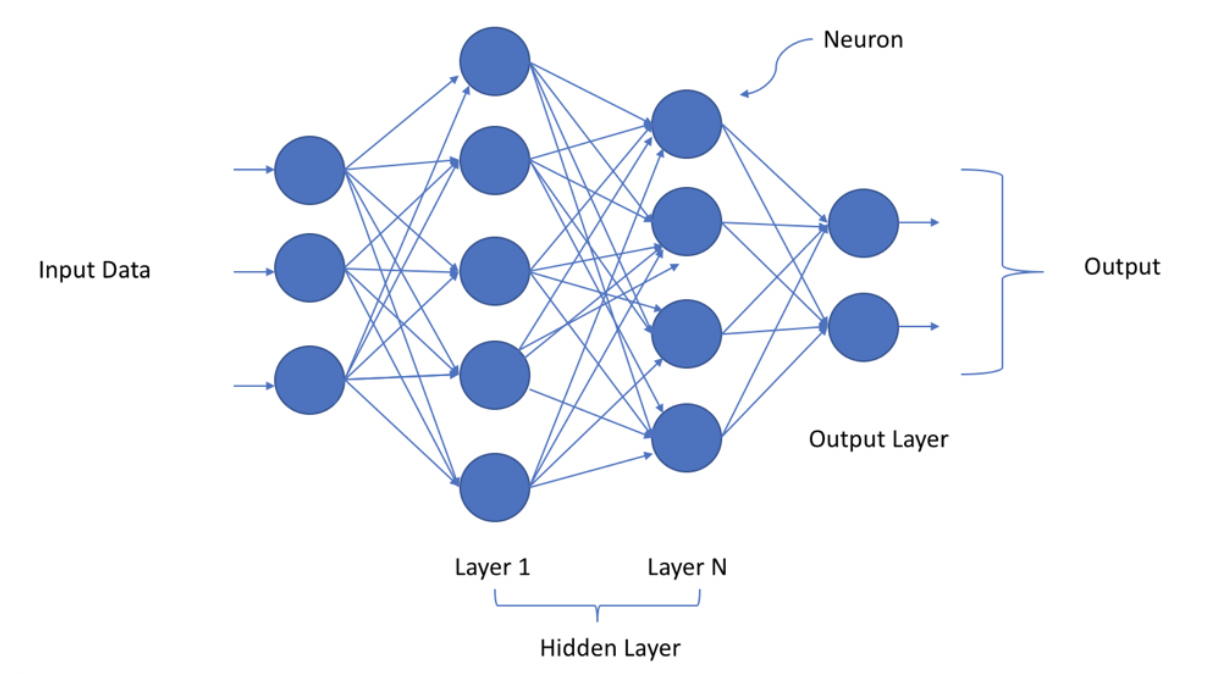
\includegraphics[width=0.95\textwidth]{DNN.png}
            \caption{Deep Neural Network (DNN) basic architecture.}
            \label{fig:dnn}
        \end{figure}
        
Deep neural networks (DNN) are artificial neural networks with multiple hidden layers. A layer is composed of a set of neurons connected to neurons from previous layer. They perform a computation and output a single value sent to the next layer. The neurons together form the neural network. A representation of a deep neural structure can be found Fig. 1.1. By combining all the neurons into a coherent ensemble, the neural network should be able to learn complex functions to solve complex problems.
Mathematically, for a set of n-1 input values $x_1, x_2, .., x_n$ a neuron will compute the following output:
\[\ out = \sigma( \sum_{i=1}^{n}{x_i \omega+ b })\]
with $\sigma(.)$ a non-linear activation function, $b$ the bias and $w_i$ the weights of the neuron. An illustration of a single neuron is presented in Fig. 2.1. To train a neural network, we tune the weights (or parameters) and bias of all neurons in order to produce a specific function.

\begin{figure}[!h]
            \centering
            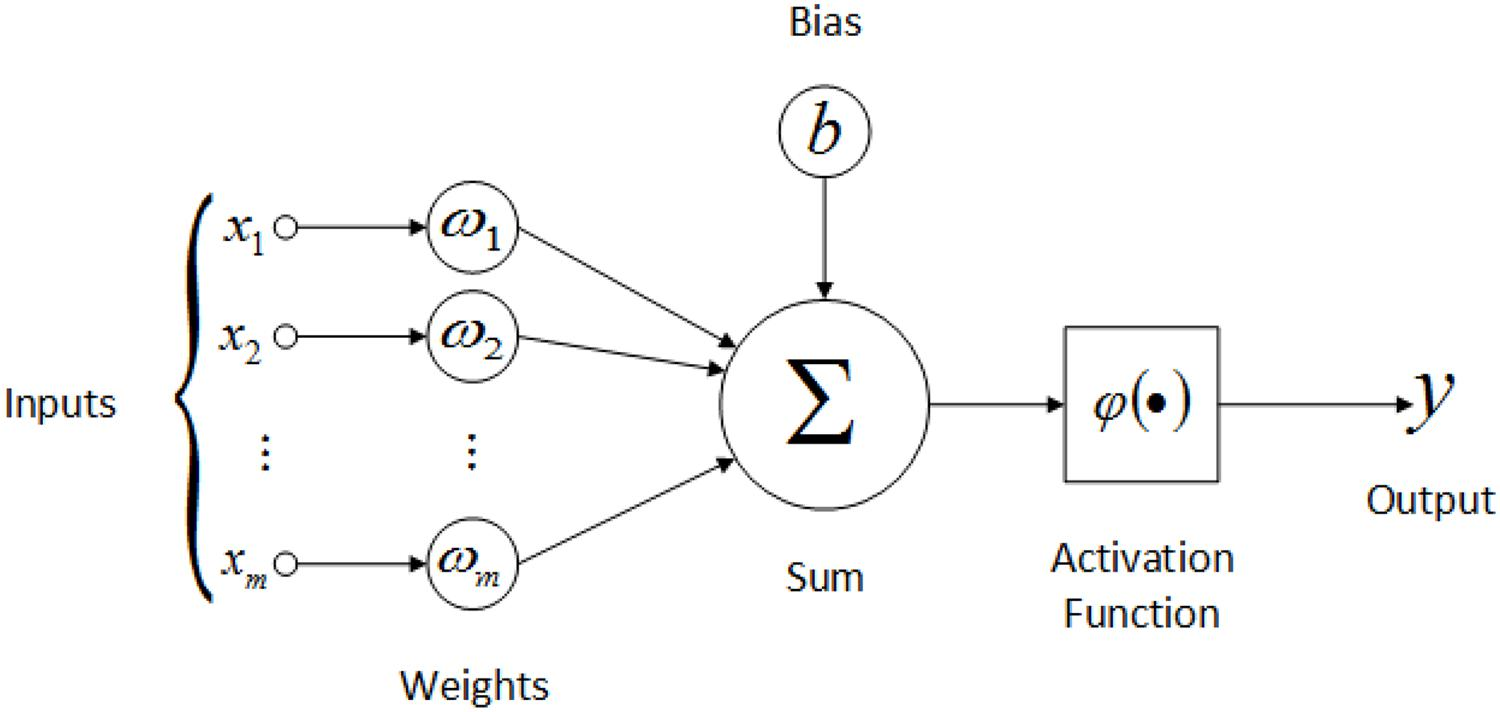
\includegraphics[width=0.55\textwidth]{MLP}
            \caption{Neuron in DNN}
            \label{fig:mlp}
        \end{figure}
        
The input layer of the neural network receives data for training which comes in different formats like images, audio, or texts. From the dataset, input features with weights and biases are used to calculate the linear function. Then, this resultant from the linear function is used by the activation function as input and calculated activations are further fed as input to the next layer.
There several types of activation functions that can be chosen by the context, the most used are the following: Sigmoid function, TanH function, ReLU function \cite{act_function}.
\newline \newline
Basically, three important steps took place in a single iteration of deep neural architectures: Forward Propagation, Backward Propagation, and Gradient Descent(Optimization).
\begin{itemize}
\item Forward Propagation: In this step input data is fed in the forward direction through each layer of the neural network. The linear calculation takes place in this step and the activation function is applied.
\item Back Propagation: This step helps in calculating all the derivatives which will be further used for Optimization or updating the parameters.
\item Optimization: This step helps in the convergence of the loss function by continuously updating the parameters in each iteration. Some optimization algorithms are as follows: Gradient Descent, Momentum, Adam, AdaGrad, RMSProp, etc.
\end{itemize}
We explained that weights and biases are the parameters that need to be changed for the network to learn, but we never mentioned if they should be increased or decreased, and by which amount. These issues are indirectly answered by the implementation of a loss function, a mathematical equation that connects all possible network variables into a single value representing the distance from the perfect performance, or how much the system is “losing” from its optimal state. When the network has poor accuracy, the loss function assumes a relatively high value, which gradually decreases as the system learns, ideally reaching zero at the end of training. The choice of a loss function is one of the most critical decisions that fall on the programmer’s shoulders, because an inappropriate one can have on the network effects extremely different from the ones intended. 


\section{From deep learning to continual learning}
Humans have the extraordinary ability to learn continually from experience. Not only can we apply previously learned knowledge and skills to new situations, we can also use these as the foundation for later learning. One of the grand goals of AI is building an artificial continual learning agent that constructs a sophisticated understanding of the world from its own experience through the autonomous incremental development of ever more complex skills and knowledge \cite{ring}.
\newline \newline
However, the learning algorithms suffer from many shortcomings. An important restriction of deep learning is the dependence on the quality of the data sets, a clean and well-built dataset being a critical condition to an effective learning process. In most machine learning algorithms, training data are assumed to be independent and identically distributed (iid), i.e. the data distribution is assumed static. If the data distribution changes while learning, the new data will interfere with current knowledge and erase it. This phenomenon is so important and it so drastically challenges the algorithms’ performance that we call it “catastrophic forgetting” \cite{cat_forgetting}. This problem has many implications in the way algorithms train neural networks and in the potential application fields for machine learning.
Let us consider, for example, a robot working in an evolving environment and being assigned the goal of manipulating new objects or solving new tasks. The robot will then need to incrementally learn new knowledge and skills to improve and adapt its behaviour to new situations. With classical machine learning techniques, in order to incorporate new knowledge while avoiding catastrophic forgetting, the model will have to re-learn everything from scratch. A robot which needs only the new data to improve and develop knowledge and skills, would be much more efficient in this situation.
\newline \newline
However, artificial learning systems today seems very far from that goal. While during the last few years we have witnessed formidable progress in the context of semi-supervised and reinforcement learning (i.e. being able to operate with less and less direct supervision) with the ability to learn more autonomously \cite{goodfellow, lecun,mnih}, very little has been done in deep learning with the idea of learning continuously.
\newline \newline
Continual learning (CL) is a branch of machine learning aiming at handling this type of situation and more generally, settings with non-iid data sources. It aims at creating machine learning algorithms able to accumulate a set of knowledge learned sequentially. The general idea behind continual learning is to make algorithms able to learn from a real-life data source. In a natural environment, the learning opportunities are not simultaneously available and need to be processed sequentially. Learning from the present data and being able to continue later with new data rather than learning only once for all, seems very appropriate. It opens the possibility to improve the algorithms on a certain task or to make them learn new skills/knowledge without forgetting. It also enables transfer between learning experiences. Previous knowledge acquired may help in learning to solve new problems and new knowledge which may improve the solutions found for past tasks. Nevertheless, because of the catastrophic forgetting phenomena, learning continually is a challenging discipline. The strategy consisting in saving everything to avoid any forgetting is not satisfying because it would not be scalable in terms of memory and computation. The amount of memory used might grow too fast. It is therefore important to remember only the essential concepts. Moreover, to deal with catastrophic forgetting, algorithms should identify the potential source of interference between tasks1 to come up with a smoother forgetting process.
\newline \newline
In technical field, here are several examples of settings where continual learning is necessary:
\begin{itemize}
\item You have a trained model, you want to update it with new data but the original training data was discarded or you do not have the right to access it any longer;
\item You want to train a model on a sequence of tasks but you can not store all your data or you do not have the computational power to retrain the model from all data (e.g., in an embedded platform);
\item You want an agent to learn multiple policies but you do not know when the learning objective changes nor how;
\item You want to learn from a continuous stream of data that may change through time but you do not know how and when.
\end{itemize}


\section{Introduction to case study: Continual learning strategies on audio classification}
In recent years Continual Learning is becoming increasingly important in the evolution of Artificial Intelligence. As will be detailed in the next chapter, CL is a branch of the machine learning that can be considered very powerful and suited for many areas. While not already as its explosion, this concept has been getting more and more attention on the Deep Learning community in the last years very good contributions have come out \cite{hoiem, Kirkpatrick}.
A lot of research has been done as this is a very avant-garde new scenario; most of them are based about image recognition and classification, it’s obviously a good start point to discuss and elaborate a new concept.
\newline \newline
In this thesis I want to focus on Audio Classification inside this new evolved concept of deep learning. This can be very interesting because the application of the concept of learning continually on the data like audio or sounds is enough appropriate: just think to the characteristics of this type of data, it can easily change over time and it’s difficult that it is linear and always similar.
Audio classification is a well-studied research field \cite{zhang} with a wide variety of applications such as multimedia search and retrieval \cite {gemmeke}, urban sound monitoring \cite{bello}, bioacoustic monitoring \cite{salamon} and audio captioning \cite{drossos}. Most recent audio classification methods employ a standard supervised learning approach applied to deep neural net- works. While successful, this approach has two significant draw- backs: it requires large quantities of labeled data and can only detect classes that were included in these data, i.e., it imposes a fixed class vocabulary. These requirements, while seemingly innocuous, can make a majority of audio classification methods unusable for applications where the target class vocabulary is not known a priori. That is, many real-world scenarios require us to customize the class vocabulary, such as adding new classes, for example, to personalize the wake-up-words on smart devices, to monitor new bird species at different locations, or to transcribe rare musical instruments.
\newline \newline
The application of continual learning in this field will not maintain the training data class vocabulary, requiring manual labeling of all novel classes for deployment, which can be overwhelming for large vocabulary problems.
This thesis aims to provide an extended perspective on the areas of application of lifelong learning and insights into the benefits of these approaches for lifelong learning.

Some of the continuous learning strategies are applied to rank the event audio on the benchmark created by a specific audio data set, which is particularly suitable for this type of classification. In addition, a broad discussion is proposed on the evaluation of these strategies, using different metrics suitable for continuous learning. 

\section{Thesis structure}
From a high-level, this thesis is divided into two parts. The first part, which ranges from Chapter \ref{chap:2} to Chapter 5, introduces the reader to the theoretical concepts needed in order to understand the second part, where main ideas are developed and evaluated. The latter starts from Chapter 6 and ends with Chapter 8. Last chapter is dedicate to the conclusion and introducing new further and possible works from the starting work discussed in this thesis.
The contributions of this thesis are:
\begin{itemize}
\item A global overview of the continual learning research field (chapter \ref{chap:2}). We present the state of the art in continual learning and introduce some definitions and notions. There are also a focus on the continual learning scenarios introducing some of them that will be used in the experiments. In the same chapter there is also a part dedicated to an overview for all different possible strategies and different metrics that allow to test and evaluate previous algorithms. Some challenges of this field are introduced in this section .
\item An implementation section that shows how a continual learning benchmark was built using two different scenarios, introduced in the first part. Then, there is a focus on three different continual learning strategies that are adopted to make some experiments on the created benchmark that will be evaluated. There is also a brief preview about audio classification and its main characteristics that allow to understand how manage this type of data. In this section there is also a main important chapter where Avalanche is introduced. It is a CL python library that help to make effective and practical experiments in continual learning field.
\item An evaluation section where every continual learning strategies is tested for different scenarios. This testing part is performed by using Avalanche library. Here there is a discussion about the results found through experiments made during this thesis work
\item Final section where conclusions are written about the work done and a focus on further works that it's possible to explore. As it said at the start of the thesis, Continual Learning is novel concept that will evolve in next years in all field, from image, audio to audio and sounds.
\end{itemize}

\part{Fundamentals}


\chapter{Continual learning}
\label{chap:2}
In the previous chapter, we introduced classical deep learning basic concepts and pipeline and showed their lack of adaptability in practical situations. We also introduced how continual learning aims at solving those shortcomings. In this chapter, we present the continual learning research field more extensively. All theoretical notions and definitions about this framework are introduced in this chapter. 
\section{Definition of Continual Learning}
Given a potentially unlimited stream of data, a Continual Learning algorithm should learn from a sequence of partial experiences where all data is not available at once. A non-continual learning setting would then be when the algorithm can have access to all data at once and can process it as desired. Continual learning algorithms may have to deal with imbalanced or scarce data problems \cite{drossos}, catastrophic forgetting \cite{sprechamn} or data distribution shifts \cite{gepperth}.

Continual Learning is based on the simple, yet fundamental idea of learning continually over time \cite{chen-2018, ring}. The basic intuition is that data are not aprioristically available, like generally assumed in machine learning research, but only in a time- delayed fashion.

This framework, also referred to as Lifelong or Incremental Learning, can be considered as a challenging research problem. 

\section{Brief History and motivation}

The concept of learning continually from experience has always been present in artificial intelligence and robotics since their birth \cite{turing,weng}. However, it is only at the end of the 20th century that it has began to be explored more systematically. Within the machine learning community, the lifelong learning paradigm has been popularized around 1995 \cite{ring,thrun-mitchell,thrun}. Since then it has been researched in four main areas: 
\begin{itemize}
    \item Continual Supervised Learning. Thrun \cite{thrun} was one of the first to study continual learning within a supervised context, where each previous or new task aims at recognizing a particular concept using binary classification.
    \item Continual Unsupervised Learning. While intuitively better suited for unsupervised learning, continual learning research in this area have not been extensive and mainly focused on topic modeling and information extraction.
    \item Continual Semi-Supervised Learning. The work in this area is well represented by the Never- Ending Language Learner (NELL) system by \cite{carloson}.
    \item Continual Reinforcement Learning. Mitchell and Thrun \cite{mithcell-thrun} first proposed some CL algorithms for robot learning which tried to capture the invariant knowledge about each individual task.
\end{itemize}


\newline \newline
As we can see, although continual or incremental learning has been proposed for more than 20 years, research in the area has not been extensive. Nevertheless it's becoming a solid interest of the machine learning and AI community only now
Continual Supervised Learning. The reasons for this delay are concentrated in some more complex and fundamental problems that have characterized AI until today.
\begin{itemize}
    \item Lack of systemic approaches: Machine learning research for the past 20 years has focused on statistical and algorithmic approaches on simple tasks (e.g., tasks where the distribution of data is assumed static). Disentangling “static” learning performance from continual learning side effects is important for the very incremental nature of the research and to facilitate comparison between approaches in this area.
    \item Limited amount of data and computational power: Digital data is a luxury of the 21st century. Before the big data revolution, collecting and processing data was a daunting task. Moreover, the limited amount of computational power available at the time did not allow complex and expensive algorithmic solutions to run effectively, especially in a continual learning setting which undoubtedly makes learning more complex by having to deal with multiple tasks at the same time, as well as having to incorporate the concept of time into the learning process.
    \item Focus on supervised learning: creating labelled data is probably the slowest and the most expensive step in most ML systems. This is why learning continuously has been for a long time not a viable and practical option.
    \item Manual engineered features and had-hoc solution: Before early 2000 and early works on representation learning creating a machine learning system would mean to handcraft features and finding had-hoc solution which may differ significantly depending on the task or domain.
\end{itemize}

The relaxation of these constraints, thanks to recent advancements and results in machine learning research, as well as the rapid technological progress witnessed in the last 20 years, have open the door for starting tackling more complex problems such as learning continually.
In the following chapters we will focus on recent continual learning developments in the context of deep learning, introducing theoretical concept and notions.
\section{State of the art}

The biggest problem faced today by continual learning algorithms is known in literature as Catastrophic Forgetting or Catastrophic Inference \cite{cat_forgetting}. Neural networks almost often trained with gradient-based optimization methods suffer dramatically from this problem, experiencing a rapid overriding of the model parameters when learning from different data distributions over time. This is why almost every recent work in the context of deep continual learning has been focusing on such a problem, one of the biggest obstacle to the adoption of AI systems that learn continually.
Contrasting catastrophic forgetting is possible in many ways, and not only through careful hyper-parametrizations or basic regularization techniques. As we will later discuss in Chapter \ref{chap:3}, many different strategies have been proposed, showing, with different degree of success, that CL can be used in complex domains like computer vision and natural language modeling \cite{parisi}. Early results in this area are promising, even though still to be proven over a long sequence of batches or tasks.

In next section there is a short review of the large number of domains in which continual learning could have an impact is here summarized. All applications that use streams of data in real-time that are not easy to store in fixed data, are the ones which would benefit the most from the integration of CL features. A list of field and applications in which this framework may be beneficial or has been applied can be found below:
\begin{itemize}
    \item Computer Vision: given the high-dimensionality and high-velocity of visual information, computer vision tasks are one of more suitable domains to prove the importance of continual learning and to actually benefit from it also from a practical point of view.
    \item Natural Language Processing & Speech Recognition: Continual learning may substantially improve the human-to-machine interaction through efficient on-device personalization/adaptation. This may not only reduce the computational burden on the server side (and improve the adaptation speed), but given the highly personal nature of the information being processed by the virtual assistants, it may also force the raw data to never leave the device.
    \item Robotics: RL Intelligent Adaptive Curiosity (RL-IAC) is one of the few examples of direct application of CL in a robotic environment for learning visual salience \cite{creaye}. However, the proposed algorithm does not use deep architectures.
    \item Internet of Things: embedded devices with highly constrained hardware resources and operating off-line (due to privacy or operational reasons) may highly benefit the introduction of more efficient learning algorithm operating on real-time data and without the need of storing them. 
    \item Machine Learning Production Systems: machine learning production systems are becoming more and more common in every organization. Being able to fast train and de- ploy new prediction models over time becomes essential to provide up-to-date and always improving services. 
\end{itemize}
\chapter{Continual learning framework}
\label{chap:3}
In this chapter, we will try to define continual learning a little more formally in a comprehensive framework and with additional constraints which allow us to understand better the experiment that will be presented in following chapters.
Drawing inspiration from the famous definition of Machine Learning by \cite{michalski}, we could try to summarize continual learning, operatively, in a single sentence as in the following definition.

A computer program can learn continually from a data stream, giving a sequence of partial experience $E_i$, a target function $h^\ast$ and performance measure P. This performance to optimize $h^\ast$ improves with more processed partial experience $E_i$.

The most important thing is that every single part of data cannot be processed multiple times and if we take them in isolation, they constitute only a partial amount of total data needed to perform the learning.

In the following sections a comprehensive and detailed framework is detailed to help distinguish and disentangle different approaches in different continual learning settings 
\section{Formal definition}
Early theoretical attempts to formalize the continual learning paradigm can be found in \cite{ring-2005}. 
To give a precise definition of this framework, it is fundamental to clearly describe the data stream, its use, the algorithm functioning, its assumed prior knowledge, and its requirements in terms of supervision, memory and computation.

Definition: Continual Learning Algorithm. In continual learning (CL) data arrives in a streaming fashion as a (possibly infinite) sequence of learning experiences S = $e_1, ..., e_n$. Given X and Y as input and output random variable respectively, let us consider D a potentially infinite sequence of unknown distributions $D={D_1,...,D_n}$ over $X x Y$,we encounter over time(hence with $ n∈[2,...,\infty))$. A continual learning algorithm $A^{CL}$ is an algorithm with the following signature:
\begin{equation}
                \forall D_i\in D, \quad    A^{CL} : \langle h_{i-1}, B_i, M_{i-1}, t_i \rangle \rightarrow  \langle h_i, M_i \rangle. 
\end{equation}

Where:
\begin{itemize}
    \item $h_i$ is the current hypothesis at timestemp i, or, in other words, the parametric model learned continually,i.e.the model learned after training on experience $e_i$.
    \item $M_i$ is an external memory where we can store previous training examples or partial computation not directly related to the parametrization of the model.
    \item $t_i$ is a task label, void if not provided. It can be used to disentangle tasks and specialize the hypothesis parameters, as it is done in \cite{lopez}.
    \item $B_i$ is the training batch of examples. Each $B_i$ is composed of a number of examples $e_i^j$ with $j \in [1,...,m]$. Each example $e_i^j \langle x_i^j, y_j^i \rangle$, where $f^i$ is the feedback signal and can be the optimal hypothesis $h^\ast(x,t)$ (i.e., exact label $y_j^i$ in supervised learning), or any real tensor (from which we can estimate $h^\ast(x,t)$, such as a reward $r_j^i$ in RL).
\end{itemize}

The objective of a CL algorithm is to minimize the loss $L_s$ over the entire stream of data $L_S$:
\begin{equation}
                L_S(h_n,n) = \frac{1}{\sum_{i=1}^{n}{|B_{test}^i|}} * \sum_{i=1}^{n}{L_{exp}(h_n,B_{test}^i)}
\end{equation}

\begin{equation}
                L_{exp}(h_n,B_{test}^i) = \sum_{j=1}^{|B_{test}^i|}{L(h_n(x_j^i),y_j^i)}
\end{equation}

where the loss $L(h_n(x),y)$ is computed on a single sample $\langle x,y \rangle$, such as cross-entropy in classification problems.






\section{Task}
A task is a learning experience characterized by a unique task label t and its target function $g_{\widehat{t}}(x) \equiv h^\ast(x, t = \hat{t})$, i.e., the objective of its learning.

It is important to note that the tasks are just an abstract representation of a learning experience represented by a task label. This label helps to split the full learning experience into smaller learning pieces.

The concept of task is essential in continual learning scenario. Disentangling the notion of task from training batch is important in CL since data are not available all at once, but may be as well related to the same learning objective $g_{\widehat{t}}$.
Different scenarios of continual learning framework depends on how the concept of task is treated; more details are introduced in next chapter.

\section{CL Scenarios}
We focus on the continual learning problem in which a single neural network model needs to sequentially learn a series of tasks. During training, only data from the current task is available and the tasks are assumed to be clearly separated. This problem has been actively studied in recent years and many methods for alleviating catastrophic forgetting have been proposed. However, because of differences in the experimental protocols used for their evaluation, comparing methods’ performances can be difficult. In particular, one difference between experimental protocols we found to be very influential for the level of difficulty is whether at test time information about the task identity is available and—if it is not—whether the model is also required to explicitly identify the identity of the task it has to solve.
We can introduce several key-setting that allow to explain different scenarios:
\begin{itemize}
\item Availability of task / Distribution labels. The ability of customize specific behavior for objective hypothesis giving label to each task. It makes the continual learning problem much easier
\item Task/Shift boundaries. It impacts the complexity of the problem
\item Experience content. It stays for the classes that we can find in experience. During batches we can fin the same, new or any classes
\item Classification problem. The type of the problem that can be unique or partitioned.
\end{itemize}



\begin{table}[h]
            \centering
            \begin{tabular}{ |c|c|c|c|c|  }
                \hline
                \textbf{Name} & \textbf{Task Labels} & \textbf{Boundaries} & \textbf{Classes} & \textbf{Problem}\\
                \hline \hline
                Class-Incremental & no & yes &  new & unique\\
                \hline
                Task-Incremental & yes & yes &  new & partitioned\\
                \hline
                Domain-Incremental & no & yes &  same & unique\\
                \hline
                Task-Free & no & no &  any & unique\\
                \hline
                Task-Agnostic & no & no &  any & partitioned\\
                
                
                \hline 
                
            \end{tabular}
            
            \caption{Key-Setting and Scenarios}
            \label{tab:vggrob}
        \end{table}

The most three relevant continual learning scenario are the following: Task-Incremental, Class-Incremental, Domain-Incremental.
\begin{table}[h]
            \centering
            \begin{tabular}{ c|c  }
                \hline
                \textbf{Scenario} & \textbf{Required at test time}\\
                \hline \hline
                Task-Incremental & Solve tasks so far, task-ID provided\\
                \hline
                Class-Incremental & Solve tasks so far, task-ID provided\\
                \hline 
                Domain-Incremental & Solve tasks so far, task-ID not provided\\
               
                
                
                \hline 
                
            \end{tabular}
            
            \caption{Key-Setting and Scenarios}
            \label{tab:vggrob}
        \end{table}
In the first scenario, models are always informed about which task needs to be performed. This is the easiest continual learning scenario, and we refer to it as task-incremental learning (Task-IL). Since task identity is always provided, in this scenario it is possible to train models with task-specific components. A typical network architecture used in this scenario has a “multi-headed” output layer, meaning that each task has its own output units but the rest of the network is (potentially) shared between tasks.
In the second scenario, which we refer to as domain-incremental learning (Domain-IL), task identity is not available at test time. Models however only need to solve the task at hand; they are not required to infer which task it is. Typical examples of this scenario are protocols whereby the structure of the tasks is always the same, but the input-distribution is changing. A relevant real-world example is an agent who needs to learn to survive in different environments, without the need to explicitly identify the environment it is confronted with.
Finally, in the third scenario, models must be able to both solve each task seen so far and infer which task they are presented with. We refer to this scenario as class-incremental learning (Class-IL), as it includes the common real-world problem of incrementally learning new classes of objects.
\subsection{CL Scenarios categorization}
Nowadays it's quite difficult provide a comprehensive and general categorization that that would be reasonable across all continual learning fields. One possible categorization is proposed by \cite{\cite}. The idea is based by how the task of the stream data is treated.
A CL scenario is a specific CL setting in which the sequence of N task labels respects a certain “task structure” over time. Depending on the task-awareness or task-agnosticism of the problem to learn, now we can define, on a more abstract level and based on the specific t signal availability, three different and common scenarios for CL based on the proposed framework:
\begin{itemize}
\item Single-Incremental-Task (SIT): $t_1 = t_2 = ... = t_N$
\item Multi-Task: $ \forall i,j \in [1, .., n], t_i \neq t_j $
\item Multi-Incremental-Task: $\exists i,j,k: t_i = t_j$ and $t_j \neq t_k$
\end{itemize}
In the following sections we discuss each scenario more in detail.
 \subsubsection{Single-Incremental-Task}
 The Single-Incremental-Task (SIT) is a very general scenario where we don’t have a different task supervised signal for every training batch. It can be considered as solving a single task, which is incremental in nature or just to be in a “task agnostic” setting where data can be treated to similar or very different data distributions over time. However, it may be useful, also in this case, to detect and recognize very different data distributions to specialize the behavior of the agent even without the external supervised notion of task.
 
 
  \subsubsection{Multi-Task}
  The Multi-Task (MT) scenario constitutes a typical setting for recent literature in CL where it is assumed to encounter a number of subsequent tasks over time, each corresponding to a different training batch with very different data distributions \cite{parisi}. While this setting is useful for assessing continual learning strategy, it may revel itself less appropriate for modeling real-word problems where we can encounter many different batches of data over time, related to the same task or encounter the same task many times over our lifetime.
  
   \subsubsection{Multi-Incremental-Task}
   The Multiple-Incremental-Task (MIT) scenario constitutes the more realistic scenario in which we consider natural to be able to exploit some supervision (like parents teaching in humans) or feedbacks about the tasks we are tackling over time. This allows the agent to learn task-related specialized behaviors as well the autonomous development of its generalization capabilities.
\subsection{Update Content Types}
This concept has the same importance of the previous categorization; they are two arguments strictly correlated.
We can consider three different Update Content Type (UCT) which may greatly impact on the complexity of the continual learning scenario. They refer to the possible kind of data contained in each training batch $B_i$:
\begin{itemize}
    \item New Instances (NI): in this case the content of the batch is characterized by new instances (i.e. examples) of the same classes encountered in the previous batches.
    \item New Classes (NC): the content of each batch $B_i$ is characterize by the presence of examples belonging to always different classes never encountered before in previous batches $B_1,...,B_{i−1}.$
    \item New Instances and Classes (NIC): this update content type constitutes the the most realistic setting where new examples of previous encountered classes but also new classes are encountered over time.
\end{itemize}

In order to exemplify the concept of Content Update Type defined in Definition 16, let us recover the aforementioned example of classification. If an algorithm learns the cat vs dogs classification problem on a dataset and then new images of cat vs dogs are provided to the algorithm, we are then in a New Instances case (NI), we have new data but no new concepts. If the new instances were of different classes (e.g. cars vs bikes) we then would face the New Concepts case (NC). The new instances and new concepts case would then have been a mix of both new images of known and new classes.
\section{CL strategies}
Nowadays there is no exist formal categorization about continual learning methodologies
While the community has not agreed yet on a shared categorization for CL strategies, we present a summary of the most popular continual learning strategies in four literature based on \cite{kemker,zenke}. There is no formal definition for each of those categories so this makes very difficult to understand if a particular algorithm or strategy belongs to one category or another so it really depends on a specific view of a researcher. it's reasonable to assume for example a a four way fuzzy categorisation:
\begin{itemize}
    \item Regularization Strategies
    \item Generative Replay Strategies
    \item Rehearsal Strategies
    \item Architectural Strategies
\end{itemize}
\begin{figure}[!h]
            \centering
            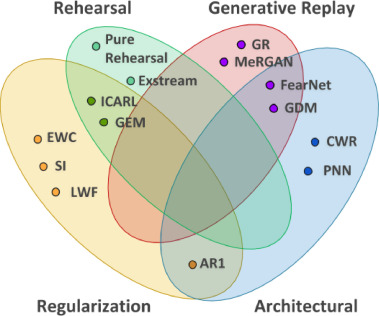
\includegraphics[width=0.65\textwidth]{cl_strategies.jpg}
            \caption{Continual learning strategies categorization.}
            \label{fig:cl_strategies}
        \end{figure}

Assuming that Rehearsal strategies can be considered also as a type of Replay strategies, we can also introduce another 3-way categorization. In the following figure different strategies are introduced under their general group. More details about them are written in next sections.

\begin{figure}[!h]
            \centering
            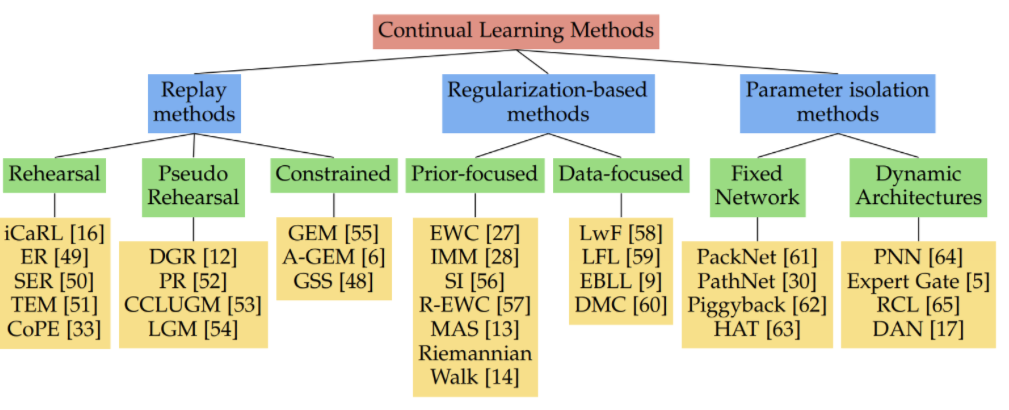
\includegraphics[width=0.8\textwidth]{cl_3strategies.png}
            \caption{Continual learning strategies 3-way categorization.}
            \label{fig:cl_strategies}
        \end{figure}
        
        
\subsection{Baseline Strategies}
Before moving to more elaborated continual learning strategies, let us consider four basic approaches:
\subsubsection{Naive} The Naive strategy simply finetunes the model across the training batches without any specific mechanism to control forgetting, except early stopping and other basic regularization techniques like L1, L2 and Dropout \cite{goodfellow-2013}, which have been already found to avoid overfitting and improve generalization. In other words it is just continue fine tuning back propagation optimization step on the new observations and new examples.
\subsubsection{JointTraining - Offline} We have a second common baseline that is a joint training or often called offline strategy. Assuming that you have access to all the data related to all the experiences at the same time, it can be considered as a pure multi-task learning
\subsubsection{Ensemble} Basically we have a separate model for each experience and we use them together doing inference for testing.
\subsubsection{Cumulative} The Cumulative strategy, also called Full Rehearsal \cite{hayes}, limits catastrophic forgetting by mixing all older examples with the new examples to be learned. When a new batch of data becomes available, there are two viable options: 
\begin{itemize}
    \item Finetuning $h_{i - 1}$ with all the cumulated patterns
    \item Start from scratch (i.e. from random weights initialization)
\end{itemize}
The cumulative learning strategy is indeed very similar to the classical multi-task training setting \cite{caruana}, which is known to yield even better performance than learning every single task in isolation.
\subsection{Rehearsal Strategies}
Rehearsal strategies are based on the idea of rehearsing past knowledge with a replay mechanism. Most of these strategies employ a fixed-sized external memory in which to store representative examples to reuse in conjunction with the new coming data in order to improve generalization without forgetting; in this way we can reuse for rehears activities that consists  in mixing those patterns with the new acquired observations and research the knowledge we have previously applied. In other words past information is periodically replayed to the model to strengthen connections for memories it has already learned. It can be defined as a simple approach that stores part of the previous training data and interleaves them with new patterns for future training. 

An example of strategy in this class is Exemplar Stream (ExStream) that was firstly introduced by \cite{hayes} as a partitioning- based method for stream clustering and the efficient management of the external fixed-size memory for rehearsal. Its performance depends on the external memory size and the task at hand.
\subsection{Generative Replay Strategies}
In this set of strategies the idea is that we do not preserve specific set of examples exactly as they are seen in the past but this approach train generative models on the data distribution. Therefore, they are able to afterwards sample data from past experience when learning on new data. By learning on actual data and artificially generated past data, they ensure that the knowledge and skills from the past is not forgotten. These methods have also been associated with the term pseudo-rehearsal \cite{robins} . A classical method implementing a generative replay normally makes use of dual models. One frozen model generates samples from past experiences and another learns to generate and classify current samples in addition to the regenerated ones. When a task is over, we replace the frozen model by the current one, freeze it, and initialize a new model to learn next task. After this definition of Generative Replay strategies, many research group this set and the previous one under the same group because both use a replay mechanism. Most of the Generative Replay based approaches are meant to solve classification tasks but there are other ones that are used for unsupervised learning or reinforcement learning.

\subsection{Architectural Strategies}
Architectural Strategies are based on the central idea of modifying the model architecture and parameters value in order to preserve old information and make space to the incoming one. Modifying connections, activation functions, freezing parameters to mitigate forgetting are very common possibilities. These strategies can be defined also dynamic because these changes to make to the architecture of a model must be done dynamically, in order to earn new concepts or skills without interfering with old ones. One of the most relevant strategy in this group is PNNs (Progressive Neural Network). 

They were originally proposed by \cite{rusu} for explicitly tackling catastrophic forgetting and are one of the best examples of the architectural category. The idea is to keep a pool of pre-trained models (or “columns”) as knowledge base, and use lateral connections between them for fast adaptation to the new batch/task.


\subsection{Regularization Strategies}
This set of strategies is based on the concept of Regularization; it is a process of introducing additional information in order to prevent overfitting. In the context of Continual Learning, the central idea is based on regularizing the learning process on the new data for preserving past learned knowledge and skills; the model should not overfit a new problem because it would make it forget it’s previous skills. The regularization approaches consist in modifying the update of weights when learning in order to keep memory of previous knowledge.
The regularization methods have been shown to be efficient in reinforcement learning \cite{Kirkpatrick}, classification \cite{chelsea} and also generative models . A limitation is that after several tasks the model may saturate because of a too high regularization, and finding a good trade-off between regularization that allows learning without forgetting may be hard.

In the following sections, most important strategies of this set are explained.

\subsubsection{Elastic Weight Consolidation (EWC)}
The Elastic Weight Consolidation (EWC) methodology alleviates catastrophic forgetting by regularizing parameters of a network trained on previous tasks by penalizing any change in them according to their importance. It can be defined as a regularization approach which tries to control forgetting by selectively constraining (i.e., freezing to some extent) the model weights which are important for the previous tasks \cite{ewc}. Intuitively, once a model has been trained on a task, thus reaching a minimum in the loss surface, the sensitivity of the model w.r.t. each of its weight $\theta_k$ can be estimated by looking at the curvature of the loss surface along the direction determined by $\theta_k$ changes. In fact, high curvature means that a slight $\theta_k$ change results in a sharp increase of the loss. A main role in this strategy is assumed by Fisher information matrix FIM \cite{fisher}. The diagonal of the Fisher information matrix F, which can be computed from first-order derivatives alone, is equivalent to the second derivative (i.e. curvature) of the loss near a minimum. Therefore, the $k^{th}$ diagonal element in F (hereafter denoted as $F_k$) denotes the importance of weight $\theta_k$. Important weights must be moved as little as possible when the model is fine-tuned on new tasks.

If we consider a sequence of tasks or batches $B_i$. After training the model on batch $B_i$ we need to compute the Fisher information matrix $F_i$ and store the set of optimal weights $\Theta^i$. $F_i$ and $\Theta^i$ will be then used to regularize the training on $B_{i+1}$. Each diagonal element $F_k^i$ can be computed as the variance of $\varphi L_{cross}(\hat{y},t)/\varphi \Theta_k$ over the $n_i$ patterns of $B_i$.

Summarizing, EWC implementation is moderately simple and, for each batch Bi, its overhead consists of:
\begin{itemize}
    \item computation of Fisher information $F^i$, requiring one forward and one backward propagation for each of the $n_i$ patterns.
    \item storage of F and $\Theta$, totaling $2m$ values, where m is the number of model weights (including biases).
   
\end{itemize}
\begin{figure}[!h]
            \centering
            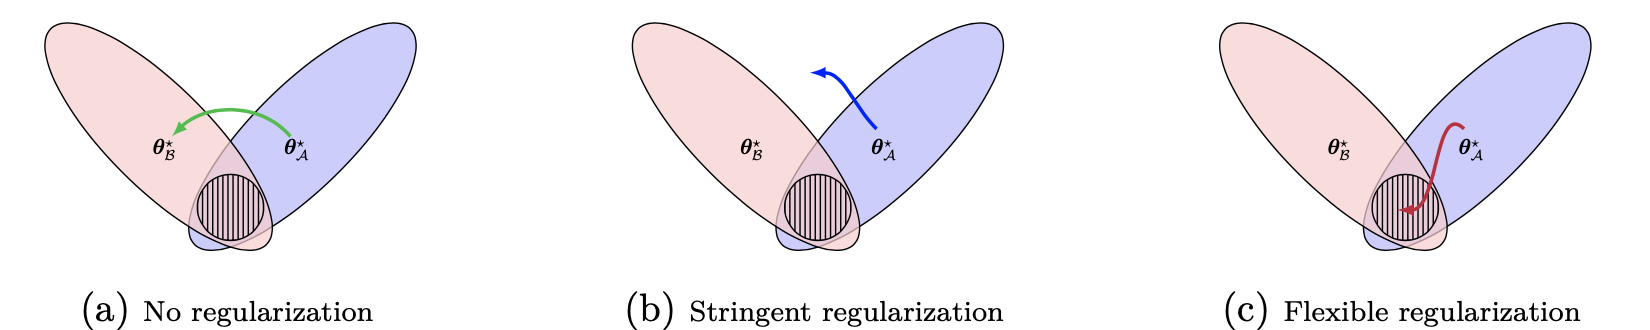
\includegraphics[width=0.95\textwidth]{ewc.png}
            \caption{Sequential training on task B after task A. (a): Train the network as it is: results in ‘Forgetting’, (b): Make no change in the parameters of previous tasks, (c): Make changes in the parameters of the previous tasks depending on their importance.}
            \label{fig:dnn}
        \end{figure}
Fig (a) represents the case when we simply fine-tune the network on the subsequent tasks. This makes the network learn the optimum parameters according to the current task, resulting in forgetting. Fig. (b) represents the case when we apply a stringent regularization to the parameters learnt from the previous tasks. This method doesn’t compute the importance of the parameters and penalizes all of them equally. This may result in the network not only forgetting the previous task, but also not be able to learn the current one. Finally, Fig. (c) refers to the EWC methodology of computing the importance of parameters before fine-tuning on new tasks. This ensures that the network learns the optimum parameters that performs well for all tasks and hence, lies in the overlapping region of the solution spaces of the tasks in the given sequence.
\subsubsection{Learning without Forgetting (LWF)}
Learning Without Forgetting (LWF) [Li and Hoiem, 2016] is a regularization approach which tries to control forgetting by imposing output (i.e. prediction) stability via distillation. It has been originally conceived for a Multi-Task (MT) setting but it can be also easily adapted to other scenario.

Distillation techniques were introduced by \cite{distillation} in order to transfer knowledge from neural network A to neural network B. The idea is that after A has learned to solve a task, we want B to share this skill with A. We then forward the same input to both A and B and impose B to have the same output as A. Distillation should be more efficient than retraining B because A produces a soft-target that helps B to learn faster. In order to apply this method for continual learning, after network A learned to solve the first task, and while B is learning the second one, we distill knowledge from A to B. In the end, B should be able to solve both tasks. A drawback of distillation is that it generally needs to preserve a reservoir of persistent data learned for each task in order to apply distillation from a teacher model to a student model
\subsubsection{Synaptic Intelligence (SI)}
Synaptic Intelligence (SI) was introduced in \cite{zenke} as a variant of EWC. The authors argued that computation of Fisher information is expensive for continual learning and proposed to calculate weight importance on-line during SGD.
SI implementation is quite simple and, for each batch $B_i$, its overhead consists of:
\begin{itemize}
    \item computation of weight importance $F^i$, based on information already available during SGD.
    \item storage of F and $\Theta$, totaling $2m$ values, where m is the number of model weights.
\end{itemize}



\part{Continual Learning benchmark for event audio classification}
\chapter{Avalanche}
\section{Brief overview}
\section{Components}
\chapter{Audio classification overview}

\section{Introduction to ESC-50 dataset}
Property of the European Southern Observatory...

\section{How perform audio classification }
\label{sec:caso}
Over the last decades, innovative observational techniques have been developed to allow spectrographs observing...

\lettrine[lines=2, findent=3pt, nindent=0pt]{I}{}n the frame of astronomical spectroscopy...

\bigskip
In \hyperref[chap:1]{Chapter~\ref*{chap:1}} we  briefly present...

\bigskip
In \hyperref[chap:2]{Chapter~\ref*{chap:2}} we summarize...


\chapter{Continual learning benchmark}

\section{Description on how build cl benchmark for audio classification using Avalanche}

\chapter{Strategies adopted}
\section{Replay}
\section{EWC}
\section{Naive}


\chapter{Avalanche implementation}

\part{Evaluating Continual Learning strategies}

\chapter{Continual learning metrics}
\section{Forgetting}
\section{BTW}
\section{Accuracy & Loss}
\section{System Metrics}

\chapter{Results }

\chapter{Discussion on the results}


\part{Conclusions}
\chapter{Conclusions \& Future works}
The grasping power of the mirror..

\backmatter
\phantomsection
\begin{thebibliography}{17}

\bibitem{Hinton-2006}
Hinton, G. E., Osindero, S., and Teh, Y.-W. (2006). \textit{A fast learning algorithm for deep belief nets. Neural Comput. 18}, 1527–1554. doi: 10.1162/neco.2006.18.7.1527

\bibitem{deep-learning}
Yann LeCun, Yoshua Bengio & Geoffrey Hinton (2015). \textit{Deep Learning}

\bibitem{neural-network}
Jürgen Schmidhuber.  \textit{Deep learning in neural networks: An overview. Neural networks,} 61:85–117, 2015.

\bibitem{act_function}
Shivam Bhardwaj (2021).  \textit{Neural Networks and Activation Function}.

\bibitem{ring}
Mark Bishop Ring. (1994)\textit{Continual learning in reinforcement environments.}

\bibitem{cat_forgetting}
Robert M. French.  \textit{Catastrophic forgetting in connectionist networks. Trends in Cognitive Sciences}, 3(4):128–135, 1999.

\bibitem{goodfellow}
Goodfellow, I., Bengio, Y., and Courville, A. (2016).  \textit{Deep Learning, volume 1.}

\bibitem{lecun}
LeCun, Y., Bengio, Y., and Hinton, G. (2015)  \textit{Deep learning. Nature,} 521(7553):436–444.

\bibitem{mnih}
Mnih, V., Kavukcuoglu, K., Silver, D., Graves, A., Antonoglou, I., Wierstra, D., and Riedmiller, M. (2013)  \textit{Playing Atari with Deep Reinforcement Learning.}
 
\bibitem{hoiem}
Li, Z. and Hoiem, D. (2016).  \textit{Learning without forgetting. In 14th European Conference on Computer Vision (ECCV 2016), volume 9908 LNCS.}

\bibitem{Kirkpatrick}
Kirkpatrick, J., Pascanu, R., Rabinowitz, N., Veness, J., Desjardins, G., Rusu, A. A., Milan, K., Quan, J., Ramalho, T., Grabska-barwinska, A., Hassabis, D., Clopath, C., Kumaran, D., and Hadsell, R. (2017). \textit{Overcoming catastrophic forgetting in neural networks.}

\bibitem{zhang}
H. Zhang, I. McLoughlin, and Y. Song. (2015). \textit{Robust sound event recognition using convolutional neural networks,} in IEEE International Conference on Acoustics, Speech and Signal Pro- cessing (ICASSP).

\bibitem{valenti}
 M. Valenti, A. Diment, G. Parascandolo, S. Squartini, and T. Virtanen (2016). \textit{Dcase 2016 acoustic scene classification using convolutional neural networks,} in Workshop on Detection and Classification of Acoustic Scenes and Events.

\bibitem{gemmeke}
J. F Gemmeke, D. P. W. Ellis, D. Freedman, A. Jansen, W. Lawrence, R. C. Moore, M. Plakal, and M. Ritter (2017). \textit{Audio set: An ontology and human-labeled dataset for audio events,} in IEEE International Conference on Acoustics, Speech and Signal Processing (ICASSP).
 
 \bibitem{bello}
 J. P. Bello, C. Silva, O. Nov, R. L. Dubois, A. Arora, J. Sala- mon, C. Mydlarz, and H. Doraiswamy (2019). \textit{Sonyc: A system for monitoring, analyzing, and mitigating urban noise pollution.} 
 
 \bibitem{salamon}
 J. Salamon, J. P. Bello, A. Farnsworth, M. Robbins, S. Keen, H. Klinck, and S. Kelling (2016). \textit{Towards the automatic classifica- tion of avian flight calls for bioacoustic monitoring.} 
 
  \bibitem{drossos}
  K. Drossos, S. Lipping, and T. Virtanen (2020). \textit{Clotho: an au- dio captioning dataset,} in IEEE International Conference on Acoustics, Speech and Signal Processing (ICASSP).

\bibitem{sprechamn}
 P. Sprechmann, S. Jayakumar, J. Rae, A. Pritzel, A. P. Badia, B. Uria, O. Vinyals, D. Hass- abis, R. Pascanu, and C. Blundell (2018). \textit{Memory-based parameter adaptation,} In International Conference on Learning Representations. 

 \bibitem{french}
 R. M. French. (1999). \textit{Catastrophic forgetting in connectionist networks. Trends in Cognitive Sciences.} 
 
 
  \bibitem{gepperth}
A. Gepperth and B. Hamme (2016). \textit{Incremental learning algorithms and applications.} 
 
   \bibitem{chen-2018}
Chen, Z. and Liu, B. (2018). \textit{Lifelong Machine Learning. Morgan & Claypool Publishers.} 


\bibitem{turing}
Turing, A. M. (1950). \textit{Computing Machinery and Intelligence.} 

\bibitem{weng}
Weng, J. (2001). \textit{ARTIFICIAL INTELLIGENCE: Autonomous Mental Development by Robots and Animals.} 

\bibitem{thrun-mitchell}
Thrun, S. and Mitchell, T. M. (1995). \textit{Lifelong Robot Learning. The biology and technology of intelligent autonomous agents.} 

\bibitem{thrun}
Thrun, S. (1996). \textit{Explanation-Based Neural Network Learning: A Lifelong Learning Approach.} 

\bibitem{carloson}
Carlson, A., Betteridge, J., Kisiel, B., Settles, B., Hruschka Jr, E. R., and Mitchell, T. M. (2010). \textit{Toward an architecture for never-ending language learning.} 

 \bibitem{mithcell-thrun}
Mitchell, T. M. and Thrun, S. B. (1993). 

\bibitem{parisi}
Parisi, G. I., Kemker, R., Part, J. L., Kanan, C., and Wermter, S. (2018). \textit{ Continual Lifelong Learning with Neural Networks.} 
 
\bibitem{creaye}
Craye, C., Lesort, T., Filliat, D., and Goudou, J.-F. (2018). \textit{Exploring to learn visual saliency.}  
 
\bibitem{michalski}
Michalski, R. S., Carbonell, J. G., and Mitchell, T. M. (2013). \textit{Machine learning: An artificial intelligence approach.}   
  
\bibitem{ring-2005}
Ring, M. B. (2005). \textit{Toward a Formal Framework for Continual Learning.}    
 
 \bibitem{lopez}
Lopez-paz, D. and Ranzato, M. (2017). \textit{Gradient Episodic Memory for Continuum Learning.}    


 \bibitem{lomonaco}
Timothée Lesort, Vincenzo Lomonaco, Andrei Stoian, Davide Maltoni, David Filliat, and Natalia Díaz-Rodríguez, (2019). \textit{Continual Learning for Robotics: Definition, Framework, Learning Strategies, Opportunities and Challenges.} 

 \bibitem{kemker}
Kemker, R. and Kanan, C. (2018). \textit{FearNet: Brain-Inspired Model For Incremental Learning.} 

  \bibitem{zenke}
Zenke, F., Poole, B., and Ganguli, S. (2017). \textit{Continual Learning Through Synaptic Intelligence.} 

 \bibitem{goodfellow-2013}
Goodfellow, I. J., Mirza, M., Xiao, D., Courville, A., and Bengio, Y. (2013). \textit{An Empirical Investigation of Catastrophic Forgeting in Gradient-Based Neural Networks.} 

 \bibitem{caruana}
Caruana, R. (1997). \textit{Multitask Learning.} 

 \bibitem{hayes}
Hayes, T. L., Cahill, N. D., and Kanan, C. (2018). \textit{Memory Efficient Experience Replay for Streaming Learning.} 
 
 \bibitem{robins}
A. Robins. (1995). \textit{Catastrophic forgetting, rehearsal and pseudorehearsal.}  
\bibitem{rusu}
Rusu, A. A., Rabinowitz, N. C., Desjardins, G., Soyer, H., Kirkpatrick, J., Kavukcuoglu, K., Pascanu, R., and Hadsell, R. (2016). \textit{Progressive Neural Networks.}     
 
 \bibitem{chelsea}
Chelsea Finn, Pieter Abbeel, and Sergey Levine. (2017). \textit{Model-agnostic meta-learning for fast adap- tation of deep networks.} 

\bibitem{ewc}
Abhishek Aich. (2021) \textit{Elastic Weight Consolidation (EWC): Nuts and Bolts.}

\bibitem{fisher}   
Jeffrey Pennington, Pratik Worah. (2018) \textit{The Spectrum of the Fisher Information Matrix of a Single-Hidden-Layer Neural Network.}

\bibitem{distillation} 
G. Hinton, O. Vinyals, and J. Dean. (2015)\textit{Distilling the Knowledge in a Neural Network.} 
\end{thebibliography}

\end{document}